% TU Berlin Beamer Template - Stand-alone Version
% https://github.com/cola4cube/beamer-theme-tub

\documentclass[aspectratio=169]{beamer}

\mode<presentation>

\usepackage[utf8]{inputenc}
\usepackage[ngerman]{babel}
\usepackage{tikz}
\usepackage{textpos}
\usepackage{calc}
\usepackage{graphicx}

\usefonttheme{professionalfonts}
\setbeamertemplate{navigation symbols}{}

% ============================================================================
% Theme Definition
% ============================================================================

\definecolor{TUred}{HTML}{C50E1F}
\definecolor{TUgrey}{HTML}{717171}
\definecolor{TUblack}{HTML}{000000}

\usecolortheme[named=TUred]{structure}

% ============================================================================
% Outer Theme
% ============================================================================

\setbeamercolor{section in head/foot}{fg=TUred,bg=white}
\setbeamercolor{subsection in head/foot}{fg=TUred,bg=white}
\setbeamercolor{author in head/foot}{parent=section in head/foot}
\setbeamercolor{title in head/foot}{parent=subsection in head/foot}

\defbeamertemplate*{title page}{customized}[1][]{}
\newcommand{\pipe}{\hspace{2pt}\textbar\hspace{2pt}}

\makeatletter
\ifdim\beamer@paperwidth=16.00cm\relax%
  \ifdim\beamer@paperheight=9.00cm\relax%
    \addtobeamertemplate{title page}{%
      \begin{tikzpicture}[remember picture,overlay]
        \node [xshift=-28.35mm,yshift=-15.04mm] at (current page.north east)
        {
\includegraphics[width=37.79mm]{TU_Logo_lang_RGB_red.png}};
      \end{tikzpicture}%
      \begin{tikzpicture}[remember picture,overlay]
        \node [xshift=80mm,yshift=9.23mm] at (current page.south west)
        {\tikz \fill [TUgrey] (0,0) rectangle (141mm,1pt);};
      \end{tikzpicture}%
      \begin{tikzpicture}[remember picture,overlay]
        \node[xshift=84.45mm,yshift=25mm,text width=150mm] at (current page.south west)
        {\usebeamerfont{title}{\color{TUred}\begin{minipage}[b][7mm][b]{141mm}
        {\inserttitle\par}\end{minipage}}\par
        {\vspace{5mm}\scriptsize{\color{TUgrey}\insertauthor \\ \insertinstitute \\ \preslocation \pipe \insertdate}}
        };
      \end{tikzpicture}
    }{}
    \defbeamertemplate*{headline}{TUBlayout}
    {%
      \vspace{4mm}
      \begin{beamercolorbox}[ignorebg,leftskip=6.45mm]{section in head/foot}
        \insertnavigation{0.5\paperwidth}\vskip2pt
        \begin{tikzpicture}[remember picture, overlay]
          \node [xshift=-21.42mm,yshift=-10.80mm] at (current page.north east)
          {
\includegraphics[width=23.94mm]{TU_Logo_lang_RGB_red.png}};
        \end{tikzpicture}%
      \end{beamercolorbox}%
    }
    \defbeamertemplate*{footline}{TUBlayout}
    {%
      \begin{tikzpicture}[remember picture,overlay]
        \node [xshift=80mm,yshift=9.23mm] at (current page.south west)
        {\tikz \fill [TUgrey] (0,0) rectangle (141mm,1pt);};
      \end{tikzpicture}%
      \begin{tikzpicture}[remember picture,overlay]
        \node[xshift=80mm,yshift=6mm,text width=141mm] at (current page.south west)
        {\scriptsize{\color{TUgrey}\insertshortauthor \pipe \insertshorttitle \pipe
        \insertdate\hfill\insertframenumber\hspace{1pt}/\hspace{1pt}\inserttotalframenumber}
        };
      \end{tikzpicture}
    }
  \fi
\fi
\makeatother

% ============================================================================
% Inner Theme
% ============================================================================

\geometry{left=0.95cm, right=0.95cm}

\setbeamercolor{frametitle}{fg=TUred,bg=white}
\defbeamertemplate*{frametitle}{customized}[1][]{}
\addtobeamertemplate{frametitle}{%
	\vspace{0pt}\hspace{0pt}\insertframetitle }

\defbeamertemplate*{toc}{customized}[1][]{}
\addtobeamertemplate{toc}{%
	\addtobeamertemplate{section in toc}{TUBlayout}{\leftskip=0.5em\large\inserttocsection\par}
}

\setbeamercolor{block title}{fg=TUred,bg=white}
\setbeamercolor{block body}{fg=black,bg=white}

\setbeamertemplate{items}[square]
\setbeamercolor{itemize item}{fg=TUred}
\setbeamertemplate{itemize item}[triangle]

\mode<all>

% ============================================================================
% Document Information
% ============================================================================

\title[Betriebssysteme]{Betriebssysteme -- Einführung}
\author[Till Zoppke]{Till Zoppke}
\institute{Studienkolleg der TU Berlin}
\newcommand{\preslocation}{Berlin}
\date{2026}

\makeindex

% ============================================================================
% Document Content
% ============================================================================

\begin{document}
  \frame[plain]{\titlepage}

% ============================================================================
\section{Geschichte}
% ============================================================================

\begin{frame}
  \frametitle{Das erste Problem: Hardware}
  \begin{columns}[T]
    \begin{column}{0.55\textwidth}
      \textbf{ENIAC (1946)}
      \begin{itemize}
        \item Electronic Numerical Integrator and Computer
        \item Programmieren durch Kabel stecken
        \item Ein Schrank = Eine Zahl speichern
        \item Rechnungen zur Wasserstoffbombe (noch klassifiziert)
      \end{itemize}
      \vspace{3mm}
      \textbf{Problem:} Umprogrammieren dauerte Tage bis Wochen
    \end{column}
    \begin{column}{0.4\textwidth}
      % ENIAC-Bild: Glen Beck und Betty Snyder programmieren den ENIAC
      % Quelle: U.S. Army Photo, Public Domain, via Wikimedia Commons
      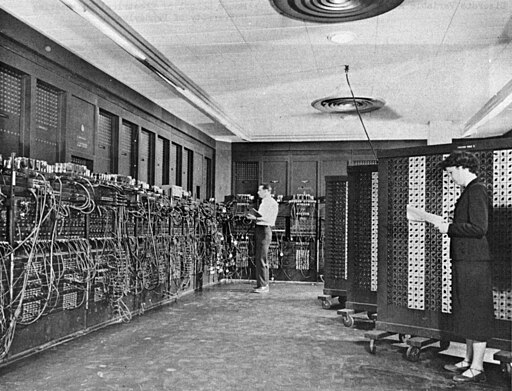
\includegraphics[width=\textwidth]{512px-Glen_Beck_and_Betty_Snyder_program_the_ENIAC_in_building_328_at_the_Ballistic_Research_Laboratory.jpg}
    \end{column}
  \end{columns}
\end{frame}

\begin{frame}
  \frametitle{Von Neumanns Transformation des ENIAC}
  \begin{columns}[T]
    \begin{column}{0.72\textwidth}
      \textbf{Die revolutionäre Idee:} Kabel bleiben gesteckt -- Befehle kommen aus dem Speicher!
      \vspace{2mm}

      \textbf{Der ``Opcode-Leser'' (Instruction Fetch):}
      \begin{enumerate}
        \item \textbf{Programmspeicher:} Die \textit{Function Tables} speicherten nun Opcodes
        \item \textbf{Befehlszähler:} Der \textit{Master Programmer} zählte Adressen statt Schleifen
        \item \textbf{Decoder:} Eine verdrahtete Schaltung aktivierte Stromkreise
      \end{enumerate}
      \vspace{2mm}
      $\Rightarrow$ So entstand \textbf{Software}: Listen von Befehlen = Programme
    \end{column}
    \begin{column}{0.25\textwidth}
      % John von Neumann - Los Alamos ID Badge
      % Quelle: Los Alamos National Laboratory, Public Domain
      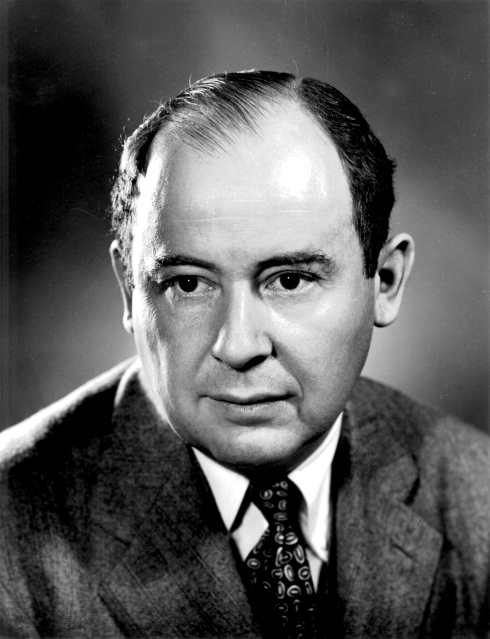
\includegraphics[width=0.95\textwidth]{JohnvonNeumann-LosAlamos.png}
      \begin{center}
        \small John von Neumann\\
        \scriptsize (1903--1957)
      \end{center}
    \end{column}
  \end{columns}
\end{frame}

\begin{frame}
  \frametitle{Die Von-Neumann-Architektur}
  \begin{columns}[T]
    \begin{column}{0.55\textwidth}
      % Von-Neumann-Architektur Diagramm
      % Quelle: Wikimedia Commons, CC-BY-SA 3.0, Autor: Medvedev
      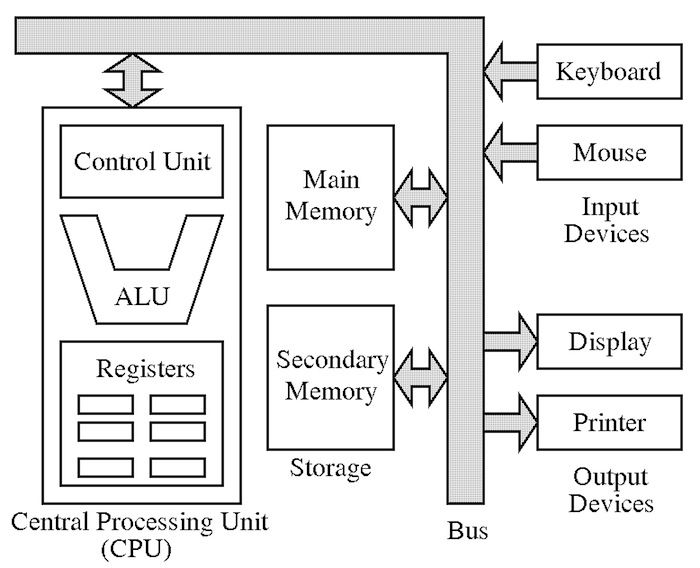
\includegraphics[width=0.9\textwidth]{vonNeumannArchitecture.jpg}
    \end{column}
    \begin{column}{0.4\textwidth}
      \vspace{2mm}
      \textbf{Kernprinzip:}\\
      Daten und Programme liegen im \textit{selben} Speicher!
      \vspace{5mm}

      \textbf{Komponenten:}
      \begin{itemize}
        \item Steuerwerk
        \item Rechenwerk (ALU)
        \item Speicher
        \item Ein-/Ausgabe
      \end{itemize}
    \end{column}
  \end{columns}
\end{frame}

% ============================================================================
\section{Speicher}
% ============================================================================

\begin{frame}
  \frametitle{Speicherhierarchie}
  \begin{center}
  \begin{tikzpicture}[scale=0.75]
    % Pyramide (schmaler)
    \fill[TUred!60] (0,4) -- (-0.7,3) -- (0.7,3) -- cycle;
    \fill[TUred!40] (-0.7,3) -- (-1.4,2) -- (1.4,2) -- (0.7,3) -- cycle;
    \fill[TUred!25] (-1.4,2) -- (-2.1,1) -- (2.1,1) -- (1.4,2) -- cycle;
    \fill[TUred!15] (-2.1,1) -- (-2.8,0) -- (2.8,0) -- (2.1,1) -- cycle;
    \fill[TUred!8] (-2.8,0) -- (-3.5,-1) -- (3.5,-1) -- (2.8,0) -- cycle;

    % Beschriftungen links
    \node[left] at (-0.7,3.5) {\small Register};
    \node[left] at (-1.4,2.5) {\small Cache (L1, L2, L3)};
    \node[left] at (-2.1,1.5) {\small RAM};
    \node[left] at (-2.8,0.5) {\small SSD / Festplatte};
    \node[left] at (-3.5,-0.5) {\small Cloud / Externe Medien};

    % Beschriftungen rechts
    \node[right] at (0.7,3.5) {\small schnell, teuer};
    \node[right] at (3.5,-0.5) {\small langsam, günstig};

    % Pfeile
    \draw[->, thick] (4,3.5) -- (4,0);
    \node[right, rotate=90] at (4.5,1.7) {\small Kapazität};
  \end{tikzpicture}
  \end{center}
\end{frame}

\begin{frame}
  \frametitle{Speicherhierarchie -- Beispiele}
  \begin{columns}[T]
    \begin{column}{0.48\textwidth}
      \textbf{ENIAC (1946):}
      \begin{itemize}
        \item Langsam: Lochkarten
        \item Schnell: Elektronenröhren
      \end{itemize}
      \vspace{5mm}
      \textbf{Standard-PC:}
      \begin{itemize}
        \item CPU-Register
        \item Cache (L1, L2, L3)
        \item RAM
        \item SSD / Festplatte
        \item Externe Festplatte
      \end{itemize}
    \end{column}
    \begin{column}{0.48\textwidth}
      \textbf{Smartphone:}
      \begin{itemize}
        \item Prozessor
        \item Level-Cache
        \item RAM
        \item Flash-Speicher
        \item Cloud
      \end{itemize}
    \end{column}
  \end{columns}
\end{frame}

\begin{frame}
  \frametitle{Diskussion: Wo sind Ihre Fotos?}
  \begin{center}
    {\Large Wo sind Ihre Fotos gespeichert?}
    \vspace{10mm}

    \textit{Tauschen Sie sich mit Ihrem Nachbarn oder Ihrer Nachbarin dazu aus.}
    \vspace{5mm}

    {\small (2 Minuten)}
  \end{center}
\end{frame}

\begin{frame}
  \frametitle{Exkurs: Backups -- Was ist das?}
  \textbf{Definition:}\\
  Ein Backup ist eine Sicherheitskopie von Daten, die bei Verlust oder Beschädigung der Originaldaten wiederhergestellt werden kann.
  \vspace{8mm}

  \textbf{Diskussionsfragen:}
  \begin{itemize}
    \item Worauf sollte man bei Backups achten?
    \item Wie sichern Sie Ihre Daten?
  \end{itemize}
\end{frame}

\begin{frame}
  \frametitle{Exkurs: Backups -- Die 3-2-1 Regel}
  \textbf{Die 3-2-1 Regel:}
  \begin{itemize}
    \item \textbf{3} Kopien Ihrer Daten
    \item \textbf{2} verschiedene Speichermedien
    \item \textbf{1} Kopie an einem anderen Ort (Offsite)
  \end{itemize}
  \vspace{5mm}
  \textbf{Fachbegriffe:}
  \begin{description}
    \item[Incremental Backup] Nur Änderungen seit letztem Backup speichern
    \item[Snapshots / Versionierung] Zustand zu einem bestimmten Zeitpunkt einfrieren
    \item[Cloud Backup] Speicherung auf externen Servern (Verschlüsselung wichtig!)
  \end{description}
\end{frame}

% ============================================================================
\section{Betriebssysteme}
% ============================================================================

\begin{frame}
  \frametitle{Warum Betriebssysteme?}
  \textbf{Historischer Kontext (1960er):}
  \begin{itemize}
    \item Computer waren groß und teuer
    \item \textbf{Time Sharing:} Mehrere Benutzer teilen sich einen Rechner
  \end{itemize}
  \vspace{5mm}
  \textbf{Aufgaben eines Betriebssystems:}
  \begin{itemize}
    \item Verwaltung mehrerer Benutzer (\textbf{Multiuser})
    \item Verwaltung mehrerer Programme (\textbf{Multitasking})
    \item Verwaltung von Hardware-Ressourcen
    \item Unterstützung von Peripheriegeräten (Treiber)
    \item Zugriffsrechte und Sicherheit
  \end{itemize}
\end{frame}

\begin{frame}
  \frametitle{Geschichte: Von Unix zu Linux}
  \begin{columns}[T]
    \begin{column}{0.5\textwidth}
      \textbf{Unix (1969--1970er):}
      \begin{itemize}
        \item Entwickelt bei AT\&T Bell Labs
        \item Ken Thompson, Dennis Ritchie
        \item In C geschrieben $\Rightarrow$ portabel
        \item Verbreitung an Universitäten
      \end{itemize}
      \vspace{3mm}
      \textbf{BSD, System V, POSIX:}
      \begin{itemize}
        \item Verschiedene Unix-Varianten
        \item POSIX: Standard für Kompatibilität
      \end{itemize}
    \end{column}
    \begin{column}{0.5\textwidth}
      \textbf{GNU-Projekt (1983):}
      \begin{itemize}
        \item Richard Stallman: ``Freie Software''
        \item Compiler, Editor, Tools -- aber kein Kernel
      \end{itemize}
      \vspace{3mm}
      \textbf{Linux (1991):}
      \begin{itemize}
        \item Linus Torvalds: freier Kernel
        \item GNU + Linux = vollständiges OS
        \item Heute: Server, Smartphones (Android), Supercomputer, IoT
      \end{itemize}
    \end{column}
  \end{columns}
\end{frame}

\begin{frame}
  \frametitle{Was ist eine Datei?}
  \textbf{Definition:}\\
  Eine Menge von Daten, gespeichert an einer bestimmten Stelle im Dateibaum.
  \vspace{5mm}

  \textbf{Typische Linux-Verzeichnisse:}
  \begin{columns}[T]
    \begin{column}{0.45\textwidth}
      \begin{itemize}
        \item \texttt{/} -- Wurzelverzeichnis
        \item \texttt{/home} -- Benutzerverzeichnisse
        \item \texttt{/etc} -- Konfigurationsdateien
        \item \texttt{/var} -- Variable Daten
      \end{itemize}
    \end{column}
    \begin{column}{0.45\textwidth}
      \begin{itemize}
        \item \texttt{/bin} -- Programme
        \item \texttt{/usr} -- Anwendungen
        \item \texttt{/tmp} -- Temporäre Dateien
        \item \texttt{/dev} -- Geräte
      \end{itemize}
    \end{column}
  \end{columns}
  \vspace{5mm}
  $\Rightarrow$ Nächste Stunde: Unix-Zugriffsrechte
\end{frame}

\begin{frame}
  \frametitle{Linux Dateibaum}
  \begin{center}
  \begin{tikzpicture}[
    level 1/.style={sibling distance=25mm, level distance=12mm},
    level 2/.style={sibling distance=20mm, level distance=12mm},
    level 3/.style={sibling distance=15mm, level distance=12mm},
    every node/.style={draw, rectangle, rounded corners, minimum width=15mm, minimum height=6mm, font=\small}
  ]
    \node[fill=TUred!30] {/}
      child {node[fill=TUgrey!20] {bin}}
      child {node[fill=TUgrey!20] {etc}}
      child {node[fill=TUred!20] {home}
        child {node[fill=TUgrey!30] {martha}
          child {node[fill=TUgrey!10, font=\scriptsize] {Dokumente}}
          child {node[fill=TUgrey!10, font=\scriptsize] {Bilder}}
        }
        child {node[fill=TUgrey!30] {till}}
      }
      child {node[fill=TUgrey!20] {var}}
      child {node[fill=TUgrey!20] {tmp}};
  \end{tikzpicture}
  \end{center}
  \vspace{3mm}
  \textbf{Beispielpfad:} \texttt{/home/martha/Dokumente/hausarbeit.pdf}
\end{frame}

\begin{frame}
  \frametitle{Multitasking}
  \textbf{Mehrere Programme ``gleichzeitig'':}
  \begin{itemize}
    \item Programme wechseln sich sehr schnell ab
    \item Zwischendrin ``schläft'' ein Programm
    \item CPU-Auslastung: Prozentuale Nutzung der verfügbaren Rechenzeit
  \end{itemize}
  \vspace{2mm}
  \textbf{Was muss verwaltet werden?}
  \begin{itemize}
    \item \textbf{RAM:} Programme teilen sich den Speicher
    \item \textbf{Register:} Belegungen werden zwischengespeichert
  \end{itemize}
  \vspace{2mm}
  \begin{center}
  \begin{tikzpicture}[scale=0.7]
    \draw[fill=TUred!30] (0,0) rectangle (1.5,0.5);
    \draw[fill=TUgrey!10] (1.5,0) rectangle (2,0.5);
    \draw[fill=TUgrey!30] (2,0) rectangle (3.5,0.5);
    \draw[fill=TUred!50] (3.5,0) rectangle (4.2,0.5);
    \draw[fill=TUgrey!10] (4.2,0) rectangle (4.8,0.5);
    \draw[fill=TUred!30] (4.8,0) rectangle (6,0.5);
    \draw[fill=TUred!50] (6,0) rectangle (6.5,0.5);
    \draw[fill=TUgrey!30] (6.5,0) rectangle (8,0.5);
    \draw[fill=TUgrey!10] (8,0) rectangle (8.5,0.5);
    \draw[fill=TUred!30] (8.5,0) rectangle (10,0.5);

    \node at (0.75,0.25) {\tiny Prog A};
    \node at (1.75,0.25) {\tiny Idle};
    \node at (2.75,0.25) {\tiny Prog B};
    \node at (3.85,0.25) {\tiny OS};
    \node at (4.5,0.25) {\tiny Idle};
    \node at (5.4,0.25) {\tiny Prog A};
    \node at (6.25,0.25) {\tiny OS};
    \node at (7.25,0.25) {\tiny Prog B};
    \node at (8.25,0.25) {\tiny Idle};
    \node at (9.25,0.25) {\tiny Prog A};

    \draw[->] (0,-0.3) -- (10,-0.3);
    \node at (5,-0.6) {\small Zeit};
  \end{tikzpicture}
  \end{center}
\end{frame}

\begin{frame}
  \frametitle{macOS Activity Monitor}
  \begin{center}
    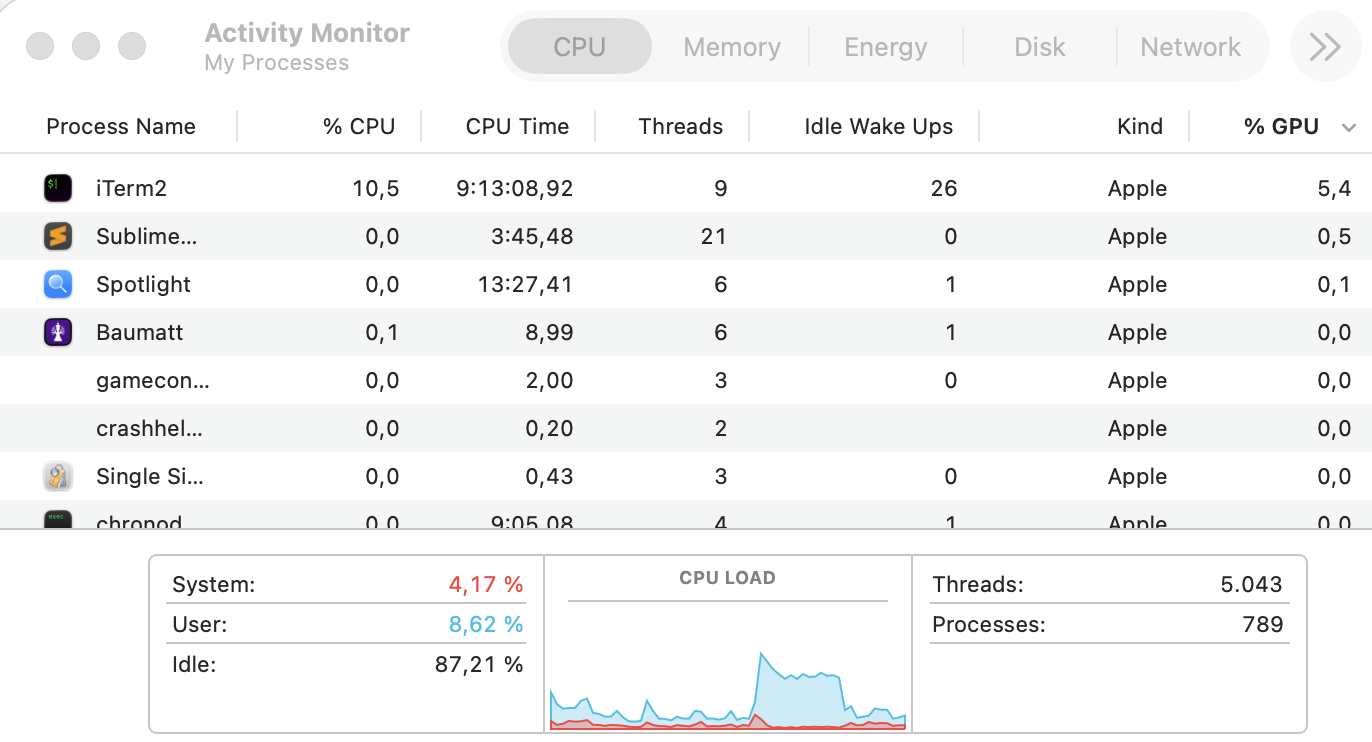
\includegraphics[width=0.75\textwidth]{activity-monitor.png}
  \end{center}
\end{frame}

\begin{frame}
  \frametitle{Prozesse mit \texttt{top}}
  \begin{center}
    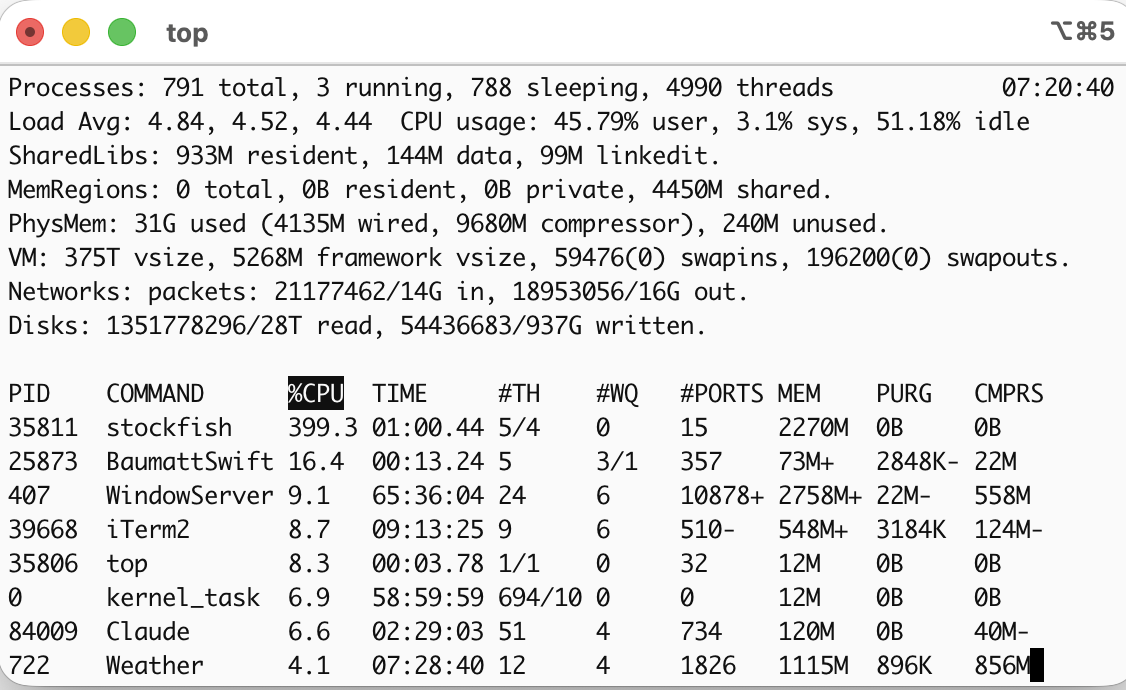
\includegraphics[width=0.65\textwidth]{top.png}
  \end{center}
\end{frame}

\begin{frame}
  \frametitle{Interrupts}
  Ein Signal, das die CPU unterbricht, um auf ein Ereignis zu reagieren.
  \vspace{4mm}

  \begin{itemize}
    \item \textbf{Hardware-Interrupts:} Mausbewegung, Tastendruck, Netzwerkpaket empfangen
    \item \textbf{Timer-Interrupt:} Regelmäßiges Signal für Prozesswechsel
    \item \textbf{Software-Interrupts:} Programm fordert Betriebssystem-Dienst an
  \end{itemize}
  \vspace{4mm}
  \begin{enumerate}
    \item Signal unterbricht aktuelles Programm
    \item CPU speichert aktuellen Zustand
    \item Betriebssystem behandelt das Ereignis (z.B. Mauszeiger neu zeichnen)
    \item Rückkehr zum unterbrochenen Programm (oder Wechsel zu anderem)
  \end{enumerate}
\end{frame}

\begin{frame}
  \frametitle{Treiber und Peripheriegeräte}
  \textbf{Frühe Computer:}
  \begin{itemize}
    \item Lochkartenleser für Dateneingabe
    \item Drucker für Ausgabe
    \item Taktgeber für Synchronisation
  \end{itemize}
  \vspace{5mm}
  \textbf{Heute: Treiber}
  \begin{itemize}
    \item Software, die Hardware ansteuert
    \item Sagt dem System, \textit{wie} eine Komponente funktioniert
    \item Beispiele: Grafikkarte, Drucker, USB-Geräte
  \end{itemize}
\end{frame}

\begin{frame}
  \frametitle{Schichtenmodell eines Betriebssystems}
  \begin{center}
  \begin{tikzpicture}[scale=0.7]
    % Schichten von unten nach oben (25% kleiner)
    \draw[fill=TUgrey!40, draw=TUgrey] (0,0) rectangle (7.5,0.75);
    \node at (3.75,0.375) {\small\textbf{Hardware}};
    \node[right, font=\scriptsize] at (7.7,0.375) {CPU, RAM, Festplatte...};

    \draw[fill=TUgrey!25, draw=TUgrey] (0,0.9) rectangle (7.5,1.65);
    \node at (3.75,1.275) {\small\textbf{Treiber}};
    \node[right, font=\scriptsize] at (7.7,1.275) {Geräte-spezifische Software};

    \draw[fill=TUred!30, draw=TUred] (0,1.8) rectangle (7.5,2.55);
    \node at (3.75,2.175) {\small\textbf{Betriebssystem-Kernel}};
    \node[right, font=\scriptsize] at (7.7,2.175) {Speicher, Prozesse, Dateien};

    \draw[fill=TUred!15, draw=TUred] (0,2.7) rectangle (7.5,3.45);
    \node at (3.75,3.075) {\small\textbf{Systemdienste / Shell}};
    \node[right, font=\scriptsize] at (7.7,3.075) {Netzwerk, Grafik, Kommandozeile};

    \draw[fill=TUgrey!10, draw=TUgrey] (0,3.6) rectangle (7.5,4.35);
    \node at (3.75,3.975) {\small\textbf{Anwendungen}};
    \node[right, font=\scriptsize] at (7.7,3.975) {Browser, Office, Spiele...};

    % Pfeile für Abstraktionsrichtung
    \draw[->, thick, TUred] (-0.6,0.375) -- (-0.6,3.975);
    \node[rotate=90] at (-1,2.2) {\scriptsize Abstraktion};
  \end{tikzpicture}
  \end{center}
  \vspace{2mm}
  Jede Schicht nutzt die Dienste der darunterliegenden Schicht.
\end{frame}

% ============================================================================
\section{Speicherverwaltung}
% ============================================================================

\begin{frame}
  \frametitle{Virtueller Speicher}
  \textbf{Prinzip:}
  \begin{itemize}
    \item Jedes Programm bekommt einen eigenen Adressraum
    \item Programme beginnen bei Adresse 0
    \item Den echten Speicherort kennt nur das Betriebssystem
  \end{itemize}
  \vspace{3mm}
  \begin{columns}[T]
    \begin{column}{0.45\textwidth}
      \textbf{Speicherbereiche:}
      \begin{itemize}
        \item \textbf{User Space:} Programme
        \item \textbf{Kernel Space:} Betriebssystem und Treiber
        \item \textbf{Gap:} Sicherheitsbereich
      \end{itemize}
    \end{column}
    \begin{column}{0.45\textwidth}
      \textbf{Fehler:}\\
      \texttt{Segmentation Fault}\\
      $\Rightarrow$ Zugriff außerhalb des erlaubten Bereichs
    \end{column}
  \end{columns}
\end{frame}

\begin{frame}
  \frametitle{Speicherlayout eines Programms}
  \begin{columns}[T]
    \begin{column}{0.4\textwidth}
      \begin{tikzpicture}[scale=0.65]
        % Kernel Space
        \draw[fill=TUred!30] (0,7) rectangle (4,8);
        \node at (2,7.5) {\small Kernel Space};
        \node[right, font=\tiny] at (4.1,7.5) {Treiber, OS};

        % Gap
        \draw[fill=TUgrey!10] (0,6) rectangle (4,7);
        \node at (2,6.5) {\small Gap};

        % Stack
        \draw[fill=TUgrey!40] (0,5) rectangle (4,6);
        \node at (2,5.5) {\small Stack $\downarrow$};

        % Shared Memory / mmap
        \draw[fill=yellow!30] (0,4) rectangle (4,5);
        \node at (2,4.5) {\small Shared Memory};
        \node[right, font=\tiny] at (4.1,4.5) {Bildschirm, libs};

        % Frei
        \draw[fill=TUgrey!5] (0,3) rectangle (4,4);
        \node at (2,3.5) {\small (frei)};

        % Heap
        \draw[fill=TUgrey!30] (0,2) rectangle (4,3);
        \node at (2,2.5) {\small Heap $\uparrow$};

        % Daten
        \draw[fill=TUgrey!50] (0,1) rectangle (4,2);
        \node at (2,1.5) {\small Daten};

        % Code
        \draw[fill=TUred!40] (0,0) rectangle (4,1);
        \node at (2,0.5) {\small Code};

        % Adressen
        \node[left, font=\tiny] at (0,0.5) {0x0};
        \node[left, font=\tiny] at (0,7.5) {0xFFFF...};
      \end{tikzpicture}
    \end{column}
    \begin{column}{0.55\textwidth}
      \textbf{Bereiche:}
      \begin{itemize}
        \item \textbf{Code:} Programmcode (nur lesen/ausführen)
        \item \textbf{Daten:} Globale Variablen
        \item \textbf{Heap:} Dynamischer Speicher (malloc)
        \item \textbf{Shared Memory:} Geteilter Speicher für Grafik, Bibliotheken
        \item \textbf{Stack:} Lokale Variablen, Funktionsaufrufe
      \end{itemize}
      \vspace{3mm}
      Ein Bereich darf entweder beschrieben \textit{oder} ausgeführt werden -- nie beides!
    \end{column}
  \end{columns}
\end{frame}

\begin{frame}
  \frametitle{Wie kommen Pixel auf den Bildschirm?}
  \textbf{Der Trick: Shared Memory}
  \begin{itemize}
    \item Programm schreibt direkt in geteilten Speicher
    \item \textbf{Compositor} liest diesen Speicher
  \end{itemize}
  \vspace{3mm}
  \textbf{Aufgaben des Compositors:}
  \begin{itemize}
    \item Window-Dekorationen (Titelleiste, Rahmen)
    \item Welches Fenster ist vorne?
    \item Teilweise überdeckte Fenster
    \item Mauszeiger zeichnen
  \end{itemize}
  \vspace{3mm}
  \textbf{Weitere Betriebssystem-Dienste:}
  Netzwerkverbindung, Dateien lesen/speichern, ...
\end{frame}

\begin{frame}
  \frametitle{Compositor -- Details}
  \begin{center}
    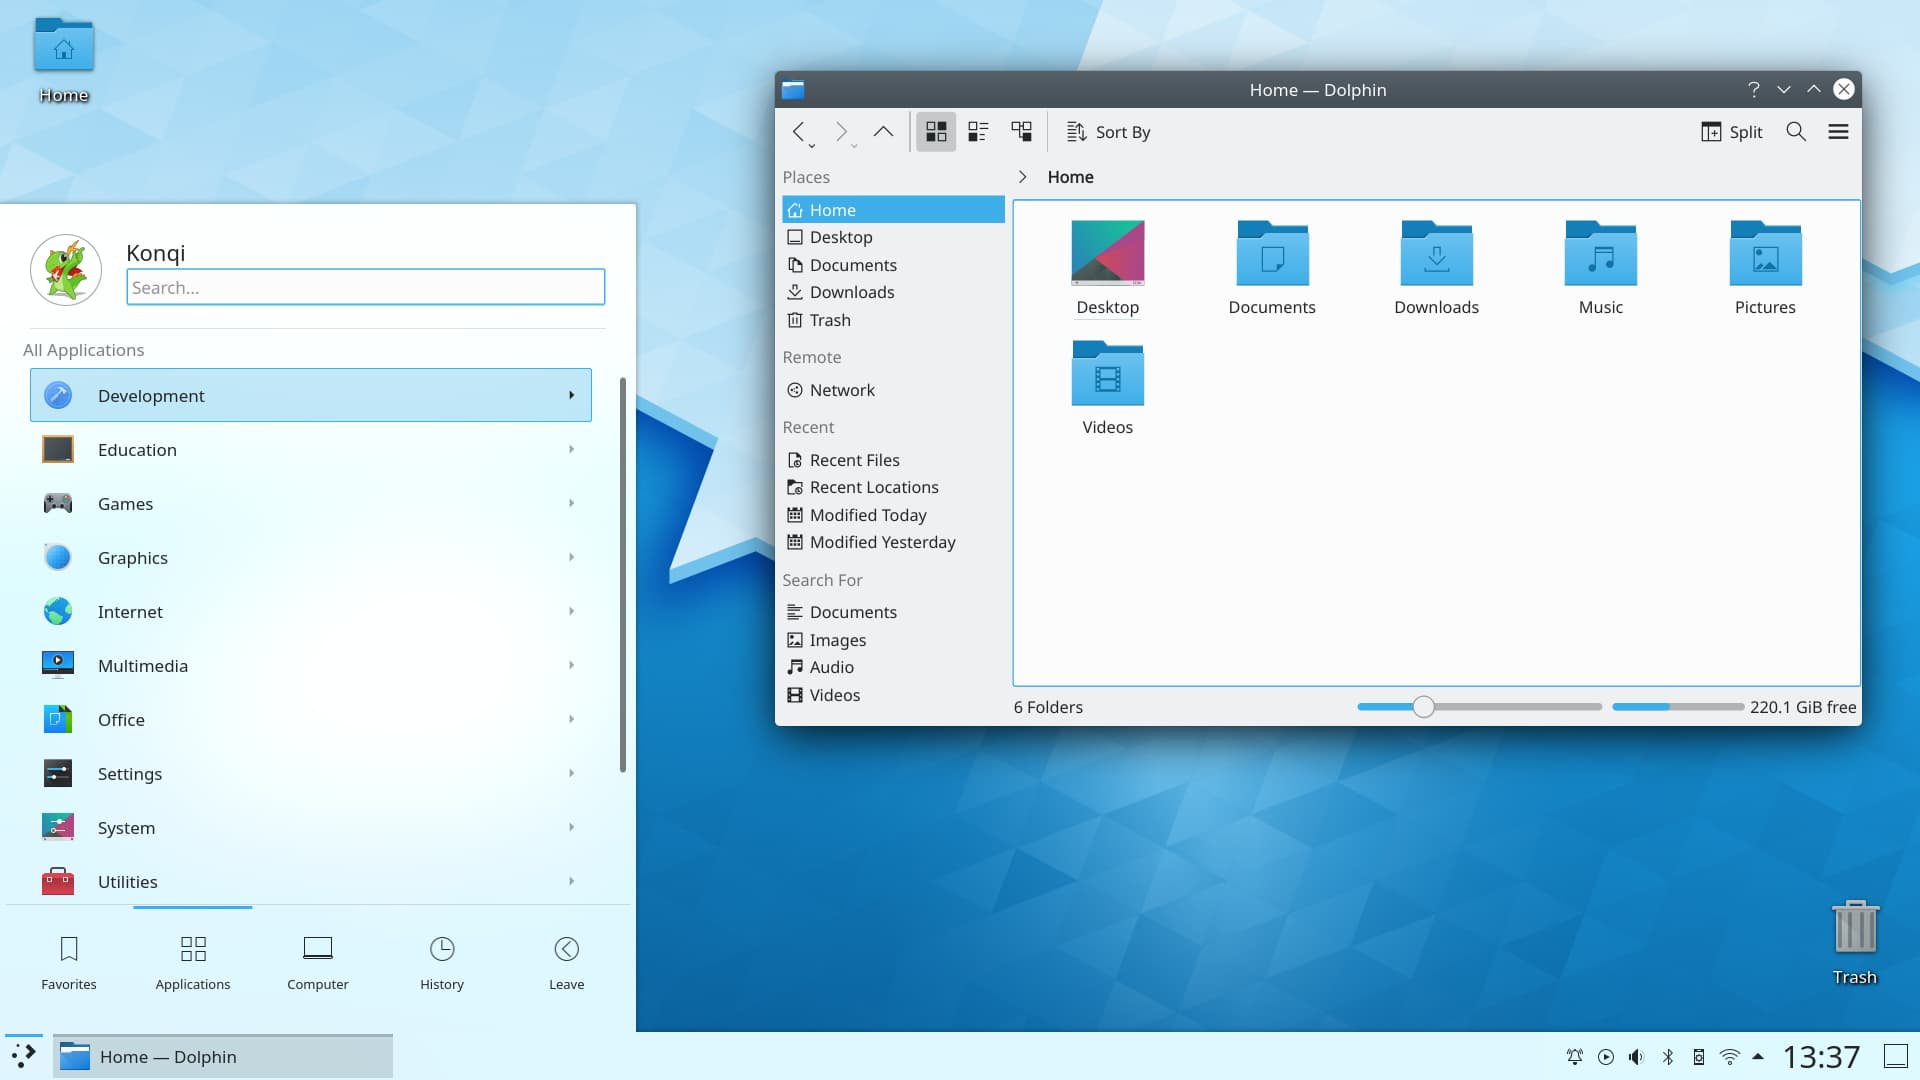
\includegraphics[width=0.7\textwidth]{screenshot-linux.jpg}
  \end{center}
\end{frame}

% ============================================================================
\section{Dateisystem}
% ============================================================================

% ============================================================================
\section{Smartphone-OS}
% ============================================================================

\begin{frame}
  \frametitle{Smartphone-Betriebssysteme}
  \textbf{Besondere Anforderungen:}
  \begin{itemize}
    \item \textbf{Immer an} -- aber trotzdem Energie sparen
    \item Teilweises Abschalten von Komponenten (CPU-Kerne, Display, Funkmodule)
    \item Schnelles Aufwachen bei Ereignissen
  \end{itemize}
  \vspace{5mm}
  \textbf{Spezielle Hardware:}
  \begin{columns}[T]
    \begin{column}{0.45\textwidth}
      \begin{itemize}
        \item Funkmodem (LTE, 5G)
        \item WLAN und Bluetooth
        \item GPS / Ortungsdienste
      \end{itemize}
    \end{column}
    \begin{column}{0.45\textwidth}
      \begin{itemize}
        \item Biometrie (Fingerabdruck, Face ID)
        \item Beschleunigungssensor, Gyroskop
        \item NFC für kontaktloses Bezahlen
      \end{itemize}
    \end{column}
  \end{columns}
\end{frame}

% ============================================================================
\section{Zusammenfassung}
% ============================================================================

\begin{frame}
  \frametitle{Zusammenfassung}
  \begin{itemize}
    \item \textbf{Von-Neumann-Architektur:} Programm und Daten im selben Speicher
    \item \textbf{Speicherhierarchie:} Schnell \& teuer $\leftrightarrow$ Langsam \& günstig
    \item \textbf{3-2-1 Backup-Regel:} 3 Kopien, 2 Medien, 1 Offsite
    \item \textbf{Betriebssystem:} Verwaltet Ressourcen, Benutzer, Programme
    \item \textbf{Schichtenmodell:} Hardware $\rightarrow$ Treiber $\rightarrow$ Kernel $\rightarrow$ Anwendung
    \item \textbf{Dateisystem:} Hierarchische Organisation von Daten
    \item \textbf{Multitasking:} Schneller Wechsel zwischen Programmen
    \item \textbf{Interrupts:} Ermöglichen Reaktion auf Ereignisse
    \item \textbf{Virtueller Speicher:} Isolation und Sicherheit
  \end{itemize}
\end{frame}

\end{document}
